\section{Database}

In this section, there are discussions about types of databases, SQL vs. NoSQL, inheritance, and conceptual schema.

A database is a~collection of data stored in a~system.
They are used for the~persistent storage of information from applications.
According to software requirements, the~data is well-organized and offers many advantages over simple file storage, such as fast search and querying.

According to~\cite{a2018_difference_db}, one of the~most critical decisions is choosing the~right type of database and the~correct database system.
Databases can be relational (SQL) and non-relational (NoSQL).

Relational databases mainly use the~SQL (Structured Query Language) language.
It is a~declarative query language that allows performing complex queries~\cite{a2018_difference_db}.
In SQL databases, data are structured, and it is based on ACID principles: atomicity, consistency, isolation, and durability.
Their scheme is fixed.
SQL databases are vertically scalable, which means increased RAM, CPU, or SSD performance.
An example of such a~database is PostgreSQL.

Non-relational databases are of many kinds and types.
They have a~dynamic schema and are suitable for hierarchic data storage~\cite{a2018_difference_db}.
NoSQL databases are horizontally scalable, allowing to handle a~more significant amount of workload by using another server.
These databases are based on CAP: consistency, availability, partition tolerance.
Examples of NoSQL databases are Neo4j and MongoDB.

Because the~data for the~developed game are with a~fixed schema, using a~SQL database is more than suitable.
The~game will use the~open-source database PostgreSQL.

\subsection{Conceptual Schema}
\label{design:conceptual}

To create a~database, creating a~conceptual schema is a~good choice.
A conceptual schema is a~schema that models only the~relations between entities.
Entities have attributes, but they do not have a~type.
An essential part of the~schema is the~relations, which can have different cardinality and partiality.

The~designed schema has six entities: \mintinline{text}|User|, \mintinline{text}|Story|, \mintinline{text}|Mission|, \linebreak\mintinline{text}|Game_mission|, \mintinline{text}|Learning_mission|, and \mintinline{text}|Game_progress|.
The~schema can be seen in the~figure~\ref{fig:design:conceptualschema}.

The~\mintinline{text}|User| entity has primary key \mintinline{text}|id| and attributes \mintinline{text}|name|, \linebreak\mintinline{text}|password|, \mintinline{text}|username|, and \mintinline{text}|description|.
The~\mintinline{text}|username| attribute is unique.

The~\mintinline{text}|Story| entity has primary key \mintinline{text}|id| and attributes \mintinline{text}|url|, \mintinline{text}|name|, and \mintinline{text}|description|.
The~\mintinline{text}|url| attribute is unique.

The~\mintinline{text}|Mission| entity has primary key \mintinline{text}|id| and attributes \mintinline{text}|url|, \mintinline{text}|name|, \linebreak\mintinline{text}|description|, and \mintinline{text}|order|.
The~\mintinline{text}|url| attribute is unique.

The~\mintinline{text}|Game_mission| entity extends entity \mintinline{text}|Mission| and has attributes \linebreak\mintinline{text}|commands_initial|, \mintinline{text}|board_initial|, \mintinline{text}|board_result|, \mintinline{text}|speed_limit|, \linebreak\mintinline{text}|robot_initial|, \mintinline{text}|robot_result|, and \mintinline{text}|task_description|.

The~\mintinline{text}|Learning_mission| entity extends entity \mintinline{text}|Mission| and has attributes \mintinline{text}|data|, and \mintinline{text}|is_story|.

The~\mintinline{text}|Game_progress| entity has primary key \mintinline{text}|id| and has attributes \mintinline{text}|commands|, \mintinline{text}|speed|, \mintinline{text}|size|, and \mintinline{text}|completed|.

From the~relations, the~\mintinline{text}|Story| entity can have multiple \mintinline{text}|Mission|s.
The~\mintinline{text}|User| entity and \mintinline{text}|Game_mission| can have multiple \mintinline{text}|Game_progress|.

\begin{figure}
    \centering
    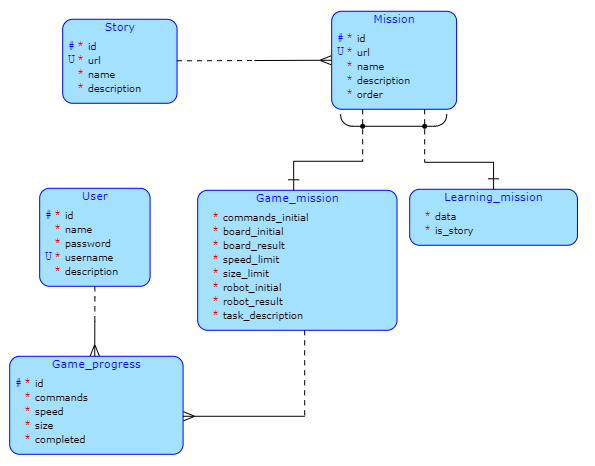
\includegraphics[width=1\linewidth]{assets/design/conceptualdiagram.png}
    \caption{Conceptual Schema}
    \label{fig:design:conceptualschema}
\end{figure}

\subsection{Inheritance}

In the~conceptual schema, inheritance is used.
Inheritance can be solved with three different approaches.

The~first approach is a~table per hierarchy~\cite{a2010_enterprise}.
This approach denormalizes the~schema and joins all tables into one.
A column that determines a~type of data is added to the~schema.
That means only one table per hierarchy is created.

The~second approach is a~table per type~\cite{a2010_enterprise}.
This approach uses tables from all entities.
There is a~foreign key to the~base table in children's tables.
Even abstract classes have their tables.
And children's tables contain only non-inherited properties.

The~third approach is a~table per concrete type~\cite{a2010_enterprise}.
This approach is similar to the~table per type, but it does not create tables for abstract classes.

Determining what approach is the~best is a~matter of specific needs.
In the~developed game, the~second approach will be used~-- the~table per type.
That means no attributes will be duplicated, and all hierarchy will be preserved.
